%%%%%%%%%%%%%%%%%%%%%%%%%%%%%%%%%%%%%%%%%
% Beamer Presentation
% LaTeX Template
% Version 1.0 (10/11/12)
%
% This template has been downloaded from:
% http://www.LaTeXTemplates.com
%
% License:
% CC BY-NC-SA 3.0 (http://creativecommons.org/licenses/by-nc-sa/3.0/)
%
%%%%%%%%%%%%%%%%%%%%%%%%%%%%%%%%%%%%%%%%%

%----------------------------------------------------------------------------------------
%	PACKAGES AND THEMES
%----------------------------------------------------------------------------------------

\documentclass{beamer}

\mode<presentation> {

% The Beamer class comes with a number of default slide themes
% which change the colors and layouts of slides. Below this is a list
% of all the themes, uncomment each in turn to see what they look like.

%\usetheme{default}
%\usetheme{AnnArbor}
%\usetheme{Antibes}
%\usetheme{Bergen}
%\usetheme{Berkeley}
%\usetheme{Berlin}
%\usetheme{Boadilla}
%\usetheme{CambridgeUS}
%\usetheme{Copenhagen}
%\usetheme{Darmstadt}
%\usetheme{Dresden}
%\usetheme{Frankfurt}
%\usetheme{Goettingen}
%\usetheme{Hannover}
%\usetheme{Ilmenau}
%\usetheme{JuanLesPins}
%\usetheme{Luebeck}
\usetheme{Madrid}
%\usetheme{Malmoe}
%\usetheme{Marburg}
%\usetheme{Montpellier}
%\usetheme{PaloAlto}
%\usetheme{Pittsburgh}
%\usetheme{Rochester}
%\usetheme{Singapore}
%\usetheme{Szeged}
%\usetheme{Warsaw}

% As well as themes, the Beamer class has a number of color themes
% for any slide theme. Uncomment each of these in turn to see how it
% changes the colors of your current slide theme.

%\usecolortheme{albatross}
%\usecolortheme{beaver}
%\usecolortheme{beetle}
%\usecolortheme{crane}
%\usecolortheme{dolphin}
%\usecolortheme{dove}
%\usecolortheme{fly}
%\usecolortheme{lily}
%\usecolortheme{orchid}
%\usecolortheme{rose}
%\usecolortheme{seagull}
%\usecolortheme{seahorse}
%\usecolortheme{whale}
%\usecolortheme{wolverine}

%\setbeamertemplate{footline} % To remove the footer line in all slides uncomment this line
%\setbeamertemplate{footline}[page number] % To replace the footer line in all slides with a simple slide count uncomment this line

%\setbeamertemplate{navigation symbols}{} % To remove the navigation symbols from the bottom of all slides uncomment this line
}

\usepackage{graphicx} % Allows including images
\usepackage{booktabs} % Allows the use of \toprule, \midrule and \bottomrule in tables

%----------------------------------------------------------------------------------------
%	TITLE PAGE
%----------------------------------------------------------------------------------------

\title[EDP Hiperbólica]{Ecuación Diferencial Parcial Hiperbólica} % The short title appears at the bottom of every slide, the full title is only on the title page

\author{Hernadez, R. J. Muñoz, F.} % Your name
\institute[UdeA] % Your institution as it will appear on the bottom of every slide, may be shorthand to save space
{
Universidad de Antioquia \\ % Your institution for the title page
\medskip
\textit{} % Your email address
}

%\date{\today} % Date, can be changed to a custom date

\begin{document}

\begin{frame}
\titlepage % Print the title page as the first slide
\end{frame}

\begin{frame}
\frametitle{Contenido} % Table of contents slide, comment this block out to remove it
\tableofcontents % Throughout your presentation, if you choose to use \section{} and \subsection{} commands, these will automatically be printed on this slide as an overview of your presentation
\end{frame}

%----------------------------------------------------------------------------------------
%	PRESENTATION SLIDES
%----------------------------------------------------------------------------------------

%------------------------------------------------
\section{Definición} % Sections can be created in order to organize your presentation into discrete blocks, all sections and subsections are automatically printed in the table of contents as an overview of the talk
%------------------------------------------------

% A subsection can be created just before a set of slides with a common theme to further break down your presentation into chunks

\begin{frame}
\frametitle{Ecuación Diferencial Parcial Hiperbólica}
Una \textbf{ Ecuación Diferencial Parcial Hiperbólica (EDPH)} es una ecuación de la forma:

\begin{equation}\label{eq:onda}
    \frac{\partial^2 u}{\partial t^2}(x,t)-c^2 \frac{\partial^2 u}{\partial x^2}(x,t)=0, \hspace{0.5cm} 0<x<a, \hspace{0.5cm} 0<t<b
\end{equation}

Un ejemplo de ecuación diferencial parcial hiperbólica es la \textbf{ecuación de onda}, para la cual se considerara la solución numérica.

\end{frame}

%------------------------------------------------

\begin{frame}
\section{Condiciones de Frontera}
\frametitle{Condiciones de Frontera}
La solución de la ecuación (\ref{eq:onda}) requiere estar sujeta a unas condiciones de frontera bien definidas, como se sigue:
\begin{equation}
    u(0,t)=u(a,t)=0, \hspace{0.5cm} \text{para}\hspace{0.5cm} 0\leq t\leq b
\end{equation}
\begin{equation*}
    u(x,0)=f(x), \hspace{0.5cm}\text{para}\hspace{0.5cm} 0\leq x\leq a
\end{equation*}
\begin{equation*}
    \frac{\partial u}{\partial t}(x,0)=g(x), \hspace{0.5cm} \text{para}\hspace{0.5cm} 0<x<a
\end{equation*}


Donde $\textbf{u}$ es el  vector de desplazamiento  de una cuerda con los extremos fijos en $x=0$ y $x=a$. y la solución analítica puede ser obtenida con series de Fourier.
\end{frame}

%------------------------------------------------
\begin{frame}
\section{Diferencias Finitas}
\frametitle{Diferencias Finitas}
En general, la diferencia finita aproxima a el valor de alguna función derivable $u(x)$ en el punto $x_0$ en su dominio. 
Supongamos una función $u(x)\in C^3$. Haciendo la expansión en serie de Taylor alrededor de $\pm h $
\begin{equation*}
    u(x+h)=u(x)+u'(x)h+u''(x)\frac{h^2}{2}+u'''(x)\frac{h^3}{6}+\textbf{O}(h^4),
\end{equation*}
\begin{equation*}
    u(x-h)=u(x)-u'(x)h+u''(x)\frac{h^2}{2}-u'''(x)\frac{h^3}{6}+\textbf{O}(h^4),
\end{equation*}
Donde el error es proporcional a $h^4$. Sumando las dos ecuaciones anteriores, se tiene:
\begin{equation*}
    u(x+h)+u(x-h)=2u(x)+u''(x)h^2+\textbf{O}(h^4)
\end{equation*}
dividiendo por $h^2$, y reagrupando los términos
\begin{equation}\label{eq:Diferencias}
    u''(x)=\frac{u(x+h)-2u(x)+u(x-h)}{h^2}+\textbf{O}(h^2)
\end{equation}
El error es proporcional a $h^2$, esta es una forma de aproximación a segundo orden. 
\end{frame}
%------------------------------------------------

\begin{frame}
\section{Solución Numérica}
\frametitle{Derivación de la solución numérica a la ecuación}
De la partición del rectángulo $R={(x,t):0\leq x\leq a, 0\leq t\leq b}$ se obtiene la malla de $n-1$ por $m-1$ rectángulos con lados $\Delta x =h$ y $\Delta  t=k$, como se muestra en la figura.
Empezando en la fila inferior, en $t=t_1=0$ donde la solución es conocida y es dada por las condiciones de frontera (i.e. $u(x_i,t_1)=f(x_i)$).

Se usará el método diferencias finitas para computar las aproximaciones
\begin{equation*}
    {u_{i,j}:i=1,2,...,n}\hspace{0.3cm} \text{ en filas sucesivas para }\hspace{0.3cm} j=2,3,...m.
\end{equation*}

\begin{figure}[h]
\centering
\includegraphics[width=0.3\textwidth]{grilla.png}
\caption{\label{fig:PenduloBalistico}Malla.}
\end{figure}
\end{frame}

%------------------------------------------------

\begin{frame}
\frametitle{Derivación de la solución numérica a la ecuación}
La solución punto a punto de la malla está dado por $u(x_i,t_j)$.
\newline

Usando el método de diferencias fintas (i.e. el resultado obtenido en (\ref{eq:Diferencias})) para la  aproximación de $u_{tt}(x,t)$ y $u_{xx}(x,t)$ son:

\begin{equation}\label{eq:expt}
    u_{tt}=\frac{u(x,t+k)-2u(x,t)+u(x,t-k)}{k^2}+\textbf{O}(k^2)
\end{equation}
\begin{equation}\label{eq:expx}
    u_{xx}=\frac{u(x+h,t)-2u(x,t)+u(x-h,t)}{h^2}+\textbf{O}(h^2)
\end{equation}
El esparcimiento de la malla es constante en cada fila: $x_{i+1}=x_i+h$ y $x_{i-1}=x_i-h$, y también constante en cada columna: $t_{j+1}=t_j+k$ y $t_{j-1}=t_j-k$. 
\end{frame}

%------------------------------------------------

%------------------------------------------------

\begin{frame}
Omitiendo los términos de orden superior, y remplazando (\ref{eq:expt}) y (\ref{eq:expx}) en la ecuación (\ref{eq:onda}), se obtiene
\begin{equation*}
     \frac{u(x,t+k)-2u(x,t)+u(x,t-k)}{k^2}=c^2\frac{u(x+h,t)-2u(x,t)+u(x-h,t)}{h^2}
\end{equation*}
la cual aproxima la solución de (\ref{eq:onda}). Por conveniencia se hace la sustitución $r=ck/h$. con lo cual la expresión anterior toma la forma
\begin{equation*}
    u_{i,j+1}-2u_{i,j}+u_{i,j-1}=r^2(u_{i+1,j}-2u_{i,j}+u_{i-1,j})
\end{equation*}
Esta ecuación es empleada para hallar la fila $j+1$ de la malla, suponiendo que los términos $j$ y $j-1$ son conocidos:
\begin{equation}\label{eq:solucion}
    u_{i,j+1}=(2-2r^2)u_{i,j}+r^2(u_{i+1,j}+u_{i-1,j})-u_{i,j-1}
\end{equation}
para $i=2,3,..,n-1$

Donde es necesario que $r\leq 1$ para garantizar la estabilidad de (\ref{eq:solucion}).
\end{frame}

%------------------------------------------------

\begin{frame}
\frametitle{Iniciando Valores}
\section{Iniciando Valores}
Las dos filas iniciales, correspondientes a $j=1$ y $j=2$ deben ser suministradas para usar la relación en (\ref{eq:solucion}). Para obtener la segunda fila se hace uso de las condiciones de frontera. Fijando $x=x_i$ en la frontera, y haciendo expansión Taylor de $u(x,t)$ al rededor de $(x_i,0)$. El valor de $u(x_i,k)$ satisface
\begin{equation*}
    u(x_i,k)=u(x_i,0)+u_t(x_i,0)k+\textbf{O}(k^2)
\end{equation*}

\begin{equation*}
    u_{i,2}=f_i+kg_i \hspace{0.5cm}\text{para}\hspace{0.5cm}i=2,3,...n-1
\end{equation*}
Sin embargo, usualmente esta relación conduce a un error que se propaga a través de la malla. 
A menudo, la función de frontera $f(x)$ tiene segunda derivada $f''(x)$ en el intervalo de interés, por lo tanto resulta conveniente usar en su lugar:
\begin{equation*}
    u_{tt}(x_i,0)=c^2u_{xx}(x_i,0)=c^2f''(x_i)=c^2\frac{f_{i+1}-2f_i+f_{i-1}}{h^2}+\textbf{O}(h^2)
\end{equation*}

\end{frame}

%------------------------------------------------

\begin{frame}

la expansión Taylor de segundo orden deja el siguiente resultado:
\begin{equation*}
    u(x,k)=u(x,0)+u_t(x,0)k+\frac{u_{tt}(x,0)k^2}{2}+\textbf{O}(k^3)
\end{equation*}
aplicando la formula anterior con $x=x_i$ se obtiene
\begin{equation*}
    u(x_i,k)=f_i+kg_i+\frac{c^2k^2}{2h^2}(f_{i+1}-2f_i+f_{i-1})+\textbf{O}(h^2) \textbf{O}(k^2)+\textbf{O}(k^3)
\end{equation*}
\begin{equation*}
    u(x_i,k)=(1-r^2)f_i+kg_i+\frac{r^2}{2}(f_{i+1}-2f_i+f_{i-1}) \hspace{0.3cm}\text{para}\hspace{0.3cm}i=2,3,...,n-1.
\end{equation*}
con esta ultima relación se obtienen los valores de la segunda fila.


\end{frame}

%------------------------------------------------

\begin{frame}
\frametitle{Resultados Ejemplo 1}
\section{Resultados}
\subsection{Ejemplo}
Use el método de diferencia finita para resolver la ecuación de onda de una cuerda que vibra con extremos fijos, dada por:
\begin{equation*}
    u_{tt}(x,t)=4u_{xx}(x,t)\hspace{0.5cm}\text{para}\hspace{0.3cm}0<x<1\hspace{0.3cm}0<t<0.5
\end{equation*}
con condiciones de frontera
\begin{equation*}
    u(0,t)=0=u(1,t)\hspace{0.3cm}\text{para}\hspace{0.3cm}0\leq t\leq 0.5
\end{equation*}
\begin{equation*}
    u(x,0)=f(x)=sen(\pi x)+sen(2\pi x)\hspace{0.3cm}\text{para}\hspace{0.3cm}0\leq x\leq 1
\end{equation*}
\begin{equation*}
    u_t(x,0)=g(x)=0\hspace{0.3cm}\text{para}\hspace{0.3cm}0\leq x\leq 1
\end{equation*}
Se elige $h=0.1$ y $k=0.05$, y dado que $c=2$, entonces $r=1$ por lo tanto
\begin{equation}\label{eq:segundaFilaEjem}
    u_{i,2}=\frac{f_{i-1}+f_{i+1}}{2}\hspace{0.3cm}\text{para}\hspace{0.3cm}i=2,3,...,9
\end{equation}
sustituyendo $r=1$ en (\ref{eq:solucion}), esta toma la forma
\begin{equation}\label{eq:SolEjemplo}
    u_{i,j+1}=u_{i+1,j}+u_{i-1,j}-u_{i,j-1}
\end{equation}

\end{frame}

%------------------------------------------------

\begin{frame}
Aplicando (\ref{eq:segundaFilaEjem}) y (\ref{eq:SolEjemplo}), se obtienen los resaltados que se muestran en la tabla.
\begin{figure}[h]
\centering
\includegraphics[width=0.95\textwidth]{tablaSol.png}
\caption{\label{fig:Balistico}Valores Obtenidos.}
\end{figure}

\end{frame}
%------------------------------------------------

\begin{frame}
\begin{figure}[h]
\centering
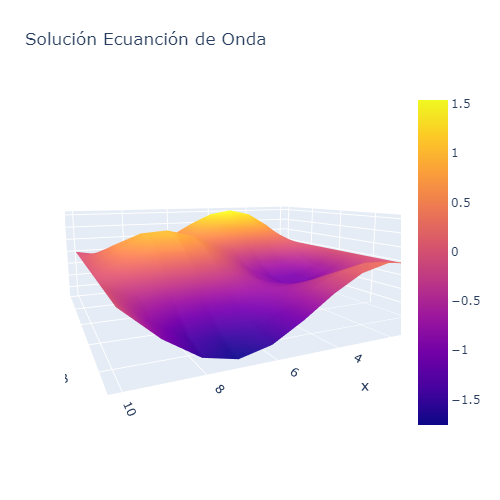
\includegraphics[width=0.5\textwidth]{OndaE1.png}
\caption{\label{fig:Pendulo}Gráfica.}
\end{figure}
Los resultados mostrados en la tabla, obtenidos numéricamente corresponden a la solución analítica dada por
\begin{equation*}
    u(x,t)=sen(\pi x)\cos(2\pi t)+sen(2\pi x)\cos(4\pi t)
\end{equation*}
Como se esperaba.
\end{frame}

%------------------------------------------------


\begin{frame}
\frametitle{Resultados Ejemplo 2}
Aproxime la solución de la ecuación de onda
\begin{equation*}
    u_{tt}(x,t)-u_{xx}(x,t)=0 \hspace{0.5cm} 0 < x < 1, \hspace{0.3cm} 0 < t;
\end{equation*}
\begin{equation*}
    u(x,0)=f(x)=\sin{2\pi x} \hspace{0.5cm} 0 \leq x \leq 1
\end{equation*}
\begin{equation*}
     u_t(x,0)=g(x)=2\pi \sin{2\pi x} \hspace{0.5cm} 0 \leq x \leq 1
\end{equation*}

\begin{figure}[h]
\centering
\includegraphics[width=0.95\textwidth]{tablaSol2.png}
\caption{\label{fig:Balistico}Valores Obtenidos Eje 2.}
\end{figure}

\end{frame}
%------------------------------------------------

\begin{frame}
\begin{figure}[h]
\centering
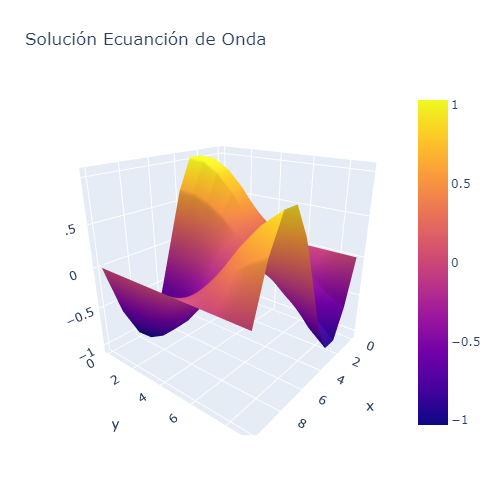
\includegraphics[width=0.5\textwidth]{OndaE2.png}
\caption{\label{fig:Pendulo2}Gráfica 2.}
\end{figure}

\end{frame}

%------------------------------------------------

\begin{frame}
\frametitle{Bibliografía}
\footnotesize{
\begin{thebibliography}{99} % Beamer does not support BibTeX so references must be inserted manually as below
\bibitem[Burden, R L. 2011]{p1} Richard L. Burden (2011)
\newblock Numerical Analysis
\end{thebibliography}
}
\end{frame}


\end{document}